\chapter{Economic aspects}
NASA scientist has published their budget in 2012 of \$18 billion, where more than 80\% of the budget was spent on robot programs and technology. The rest was spent on Cross-agency, IT, education and construction, environment, see figure \ref{fig:moneypiechartl}.
The budget covers a variety of expenses, including the rocket used to launch the spacecraft, and salaries for a team of highly skilled engineers, programmers, managers, scientists and independent contractors from around 20 states in the U.S, as well as Canada, Denmark and the U.K.\cite{EconomicNASA}.

\begin{figure}[h]
    \centering
    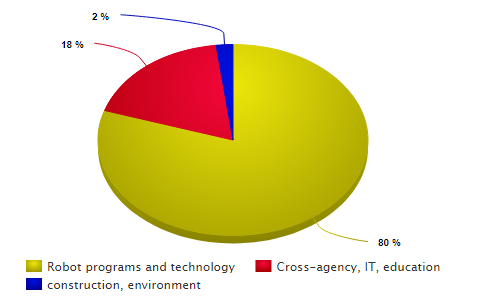
\includegraphics[[width=.8\textwidth]{figures/pieChart.png}
    \caption{NASA budget and distribution}
    \label{fig:moneypiechartl} %Make your own label so you can refer to it in the text. If you have trouble with this ask Natalie
\end{figure}

In addition to these achievements NASA is going to investigate more money on Mars rovers, exploring a deeper environment of Mars. This Project specifies a lot of time and money to send another more complicated robot to Mars.
Furthermore, Europe space agency (ESA) spend more than 5.77 billion dollars on the resources on Mars. But all preparations were unsuccessful. Despite bad projects, ESA is going to try to explore their resources in the future\cite{EconomicESA2}\cite{EconomicESA}.
